\chapter{Free Electrons}

\section{The company}
Free Electrons is an engineering company founded in 2004 by Michael Opdenacker, a Linux and Free and Open Source softwares' enthusiast. Since its beginnings, the company offers training services for development in Open Source software programs such as the Linux kernel, the Yocto Project and OpenEmbedded, Buildroot or Android. It also offers its expertise in embedded Linux development for companies willing, for example, to use Linux in their products, to upstream drivers in kernel or build a custom Linux system.

Free Electrons' team is split between two locations in France:
\begin{itemize}
  \item Orange, for General Managers and the accounting,
  \item Toulouse, for the engineering team;
\end{itemize}

Two engineers are also teleworking from Lyon's surroundings.

\section{The team}

\begin{figure}[H]
  \centering
  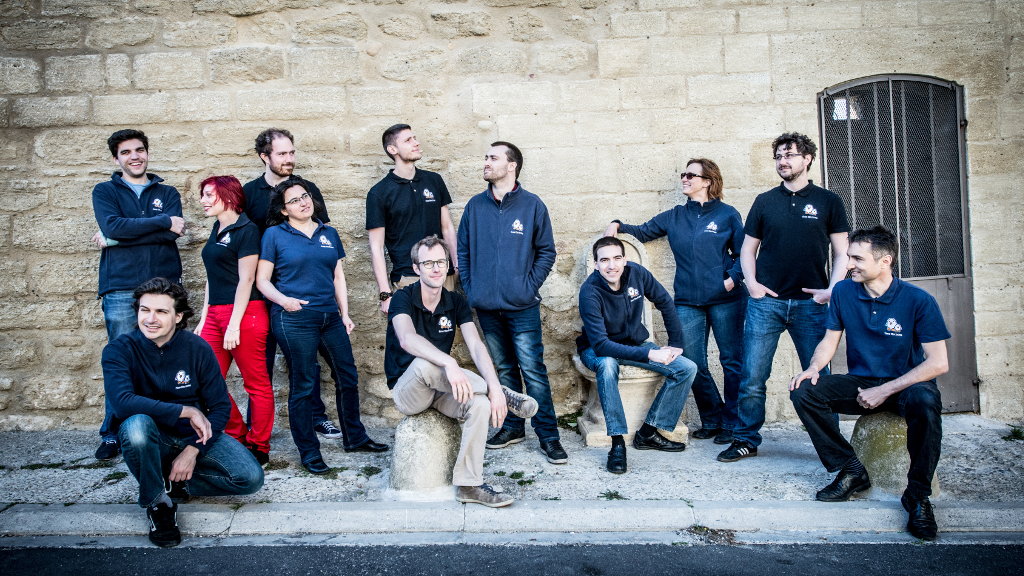
\includegraphics[width=0.866\textwidth]{free-electrons-team.png}
  \caption{Free Electrons is proud to have the conviviality of a human-size company with 11 employees and 2 interns. From left to right: Maxime Ripard, Grégory Clément, Mylène Josserand, Antoine Ténart, Maria Llvata (executive director), Quentin Schulz (intern), Thomas Petazzoni (CTO), Romain Perier, Alexandre Belloni, Anja Roubin (executive assistant), Boris Brezillon and Michael Opdenacker (founder and CEO). Florent Revest also joined Free Electrons as an intern later.}
\end{figure}

\section{Strong focus on Free and Open Source software programs}
Since its creation, Free Electrons is doing its best to contribute to the Free Software community. It does it by releasing all its training materials\footnote{\url{http://free-electrons.com/training/}} under free documentation license\footnote{\url{https://creativecommons.org/licenses/by-sa/3.0/}}. The company strongly encourages clients to share our combined work with the community and thus has a preference for clients willing to interact with and give back to the free software community by sparing some of project's time on upstreaming modifications to free software programs.

\section{A recognized expertise}
Free Electrons' engineers are well-known in communities of free software programs, such as the Linux kernel and Buildroot, thanks to their tremendous number of contributions in these different projects and also by attending and presenting talks in famous conferences around the globe, like the Embedded Linux Conference\footnote{\url{http://www.embeddedlinuxconference.com/}} or the FOSDEM\footnote{\url{https://fosdem.org}}.

\begin{figure}[H]
  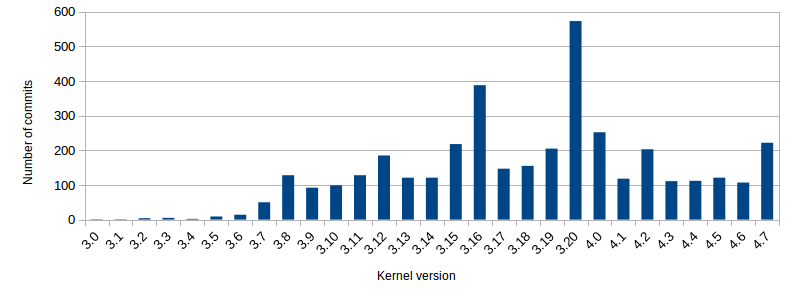
\includegraphics[width=\textwidth]{free-electrons-contributions.png}
  \caption{Free Electrons' contributions in the Linux kernel}
\end{figure}
\begin{figure}[H]
  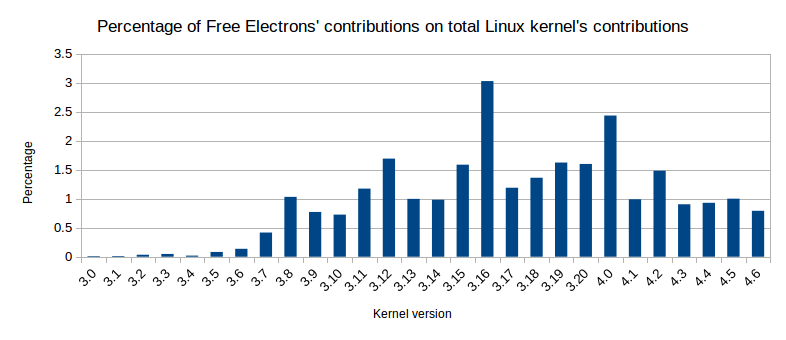
\includegraphics[width=\textwidth]{free-electrons-percentage.png}
  \caption{Percentage of Free Electrons' contributions on total the Linux kernel's contributions}
\end{figure}
\begin{figure}[H]
  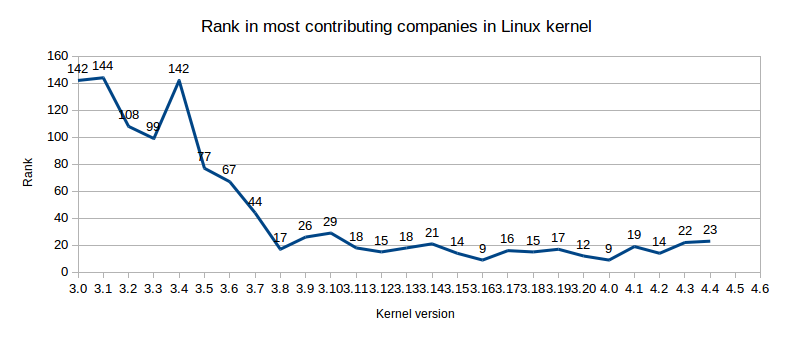
\includegraphics[width=\textwidth]{free-electrons-rank.png}
  \caption{Rank in most contributing companies in the Linux kernel}
\end{figure}

Being a big contributor often opens great opportunities in the Linux kernel. One of these opportunities is to become a maintainer of a subsystem of the kernel. The Linux kernel is such a big project that it is organized in different parts, called subsystems, and also needs maintainers which take care of a subsystem by validating code being merged to the Linux kernel source code.

Free Electrons has currently 6 maintainers\footnote{\url{https://git.kernel.org/cgit/linux/kernel/git/torvalds/linux.git/tree/MAINTAINERS}} in its engineering team:
\begin{itemize}
\item Alexandre Belloni, maintainer of ATMEL SoCs, Real-Time Clock,
\item Boris Brezillon, maintainer of NAND flash, ATMEL Clocks, Marvell cryptography driver,
\item Grégory Clément, maintainer of Marvell SoCs,
\item Thomas Petazzoni, maintainer of FBTFT Framebuffer drivers, Marvell MVNETA Ethernet driver, Marvell PCI driver,
\item Maxime Ripard, maintainer of Allwinner SoCs, Allwinner A10 DRM drivers, NVMEM framework,
\item Antoine Ténart, maintainer of Annapurna Labs architecture;
\end{itemize}

The company works with both reknown hardware vendors and companies who build custom boards which asserts Free Electrons' expertise.

We started working with NextThing Co. a year ago on one of the cheapest computer in the world\footnote{\url{https://getchip.com/}}: the C.H.I.P, sold for only 9\$ and its dedicated case embedding a touchscreen, a keyboard and a battery pack, the PocketCHIP for 69\$. Free Electrons is adding support for all the hardware components, be it the different video outputs, the camera, the NAND, the Power Management or the screen for example, in the Linux kernel and in the bootloader U-Boot.

\begin{figure}[H]
  \centering
  \begin{minipage}[b]{0.45\textwidth}
    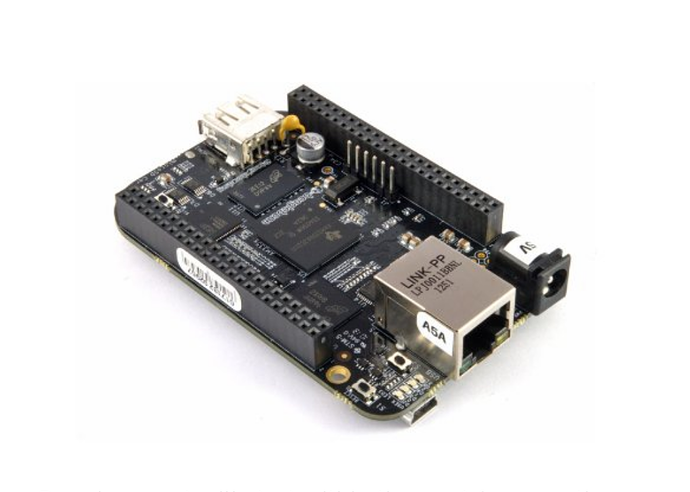
\includegraphics[width=\textwidth]{chip.png}
    \caption{C.H.I.P.: the 9\$ computer}
  \end{minipage}
  \hfill
  \begin{minipage}[b]{0.45\textwidth}
    \centerline{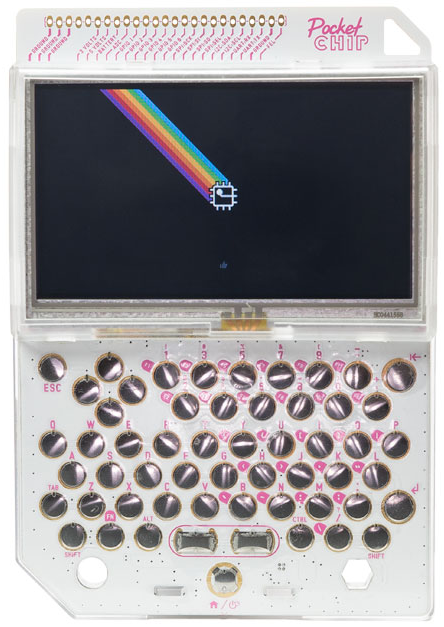
\includegraphics[width=0.7\textwidth]{pocketchip.png}}
    \caption{PocketCHIP}
  \end{minipage}
\end{figure}
